%!TEX root = thesis.tex
%% %% ***************** Background *****************

%% ************************************************ 2 ************************************************

\section{Background}\label{sec:background}

Machine learning, or ML,
is a subcategory of the AI field and data science.
Typically, ML refers to
a set of technologies used to \enquote{build computers
that improve automatically through experience}.~\cite{jordan2015machine}
This is generally considered a machine way
to simulate the human learning process.
ML usage has become more common
and is nowadays widely used in many fields,
not just in general information technology and computer science.
This is because data can be gathered from anywhere,
and where there is data to be processed,
ML can be used to process it.
Computer algorithms are able to find 
statistical correlation and patterns
from places overlooked by the human mind,
or in cases where the amount of data is just too much
for people to process.
This is why ML has proved its power
in various empirical science fields,
such as biology, cosmology or social science.~\cite{jordan2015machine}

In this section, 
key concepts of ML are explained briefly
and several ML features
that are most relevant to this study
are explored.
We also briefly discuss about data sensitivity
and how it was addressed during this study.

%% ************************************************************************************************************


\subsection{Machine learning algorithms and training}\label{subsec:bg-machine-learning}

An algorithm is a finite sequence of (typically) mathematical operations
that are used to solve a specific problem,
generally by repetition of certain steps
until the problem resolves.~\cite{merriam2022algorithm}
Algorithms are the main component inside machine learning.
By iterating through all the data points,
an algorithm is able to, for example,
find repeating patterns,
mathematical or logical connections,
or unusual anomalies that would appear seemingly normal for the human eye.

Algorithms operate on a set of rules and parameters.
In order to utilize an algorithm to solve a problem,
the algorithm is first trained by tuning these parameters
to fit the current case.
Usually,
ML algorithms can be trained in three ways:
supervised, unsupervised, and reinforcement learning.~\cite{jordan2015machine}
Even more training methods exist
that usually combine those mentioned.~\cite{ayodele2010types, mahesh2020machine}
For the sake of simplicity,
we focus only on the three main methods.

In \textbf{supervised learning},
the algorithm is given data with ready answers on
how the data needs to be interpreted.
Algorithm then tries to figure out the rules behind
how the given data and the correct answers are related.~\cite{ayodele2010types}
In \textbf{unsupervised learning},
on the other hand,
the algorithm does not get model data from which to train itself,
but instead it tries to find clusters or groups inside the data
that are linked together more closely than to other data points.~\cite{winky}
\textbf{Reinforcement learning} refers to a method
where a computer program is given a goal
and provided feedback as a reward.
This reward is what the program aims to maximize
by adjusting the parameters it has been given.~\cite{ayodele2010types}

In ML,
there are multiple algorithms to solve different problems
and no jack-of-all-trades algorithm exists.
Each algorithm is suitable for a certain type of problem.
To simplify,
algorithms are usually divided into three or four categories
based on the problem type.~\cite{vickery2019mltypes}

\textbf{Regression algorithms} predict values
and are typically used with supervised learning.
A usual example of a regression problem
is house price prediction
using typical house features
such as building
year, location, number of rooms \etc.
The algorithm then assigns each feature a weight value
which determine the final price of the house.~\cite{vickery2019mltypes}

\textbf{Classification algorithms} predict categories
and are also used most commonly with supervised learning.
Depending on the algorithm,
they can predict between two or more categories.
Examples of classification problems
could be spam mail identification with two class classification,
or flower species recognition from images with multiclass classification.~\cite{vickery2019mltypes}

\textbf{Clustering algorithms} use unsupervised learning
to find structures inside data.
This is done,
for instance,
by first providing the amount of clusters to search to the algorithm,
which then calculates a center point for each cluster
so that they are as far away from each other as possible,
while the data points surrounding each center are as close to each other as possible.~\cite{mahesh2020machine}
This could be used,
for example,
to find meaningful customer segments from transaction data
in order to improve targeted advertising.~\cite{chen2017purtreeclust}

\textbf{Dimension reduction algorithms} are a separate type of algorithms used with unsupervised learning,
but they are usually combined with other algorithms
to solve the main problem.
With dimension reduction,
main algorithm calculations are streamlined by first reducing the amount of feature dimensions.~\cite{li2017mlalgorithm}

These four ML problem types
and most known algorithms of each type
are presented in the figure~\ref{fig:ml-algorithm-cheatsheet}.


\begin{figure}[htb]
    \centering
    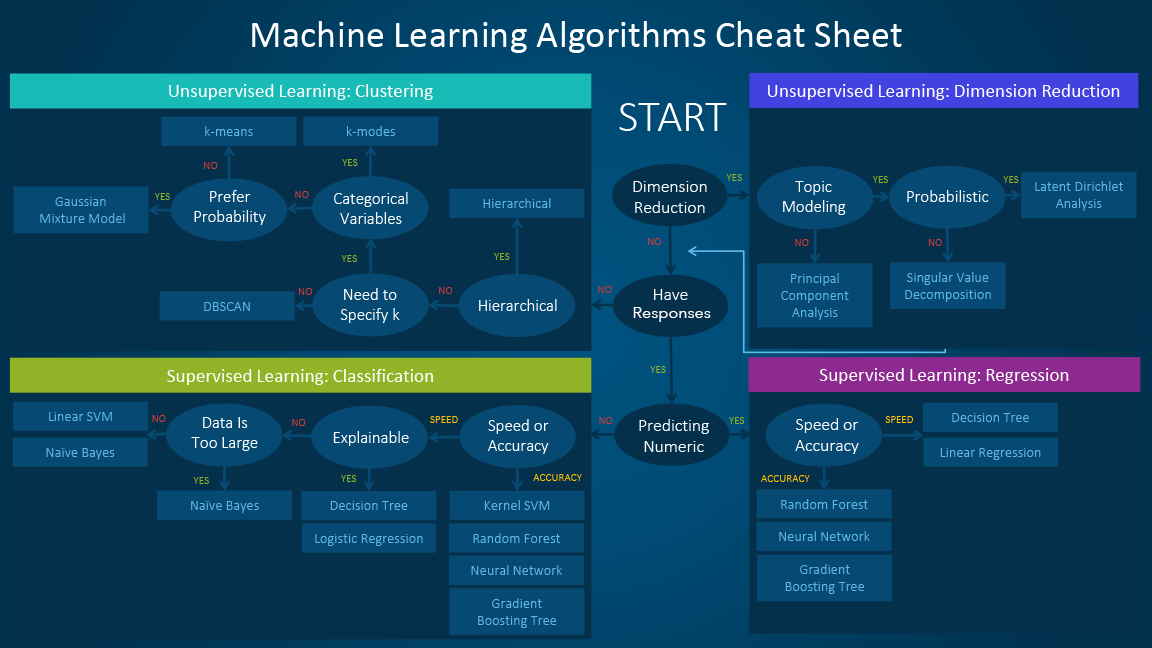
\includegraphics[width=150mm]{./appendices/machine-learning-cheet-sheet-2}
    \caption{Machine learning cheatsheet for algorithm choosing\cite{li2017mlalgorithm}
    \label{fig:ml-algorithm-cheatsheet}}
\end{figure}

This study focuses on anomaly detection,
which, simply put, is a clustering problem
where anomalies are rare incidents outside common clusters.
However,
in this study we utilize a PCA-based anomaly detection algorithm,
where PCA refers to Principal Component Analysis,
and which is a dimension reduction algorithm.~\cite{li2017mlalgorithm}
PCA is discussed in more detail later in this section.
In addition,
we aim to find a connection between anomalies and incident tickets
by their amount in a timeframe,
which makes the topic in the end a regression problem.

Typically,
the data used in algorithm training
is divided in two parts.
One part is used for the training process,
and the other is used to validate the results of the training.
These data parts must not overlap,
but the algorithm is given data to validate
that it has not seen before.~\cite{baheti2022datasplit}
For example,
in supervised learning
the key values the algorithm is trained to find
are hidden in the validation data.
The resulting values produced by the algorithm
are compared to the hidden values
and the difference between the estimate and the real value
can be used to determine how well the current trained algorithm compares to others.
However, in this study,
we are going to break that rule
of non-overlapping training and validation data.
The reason for this is explained further in section~\ref{subsec:pipe-unconventional-training}.

%% ************************************************************************************************************


\subsection{Cloud ML platforms}\label{subsec:bg-cloud-ml-platforms}

Machine learning algorithms are not light to operate.
ML is at its best with big data
where the large amount of data points
makes it easier for algorithms
to find repeating patterns more reliably.~\cite{zhou2017machine}
Data amount, however,
requires huge resources in terms of memory and computing power.
Especially with online applications
where real time analysis of new input data is required
with small latency,
cloud computing can make a big difference
in terms of processing speed.

The online market offers several solutions for ML computing in cloud.
Most notable service providers for
MLaaS (Machine Learning as a Service)
are Google, Amazon, IBM, and Microsoft.
Differences of each service provider are listed in table~\ref{fig:mlaas-comparison}.

\begin{figure}[htb]
    \centering
    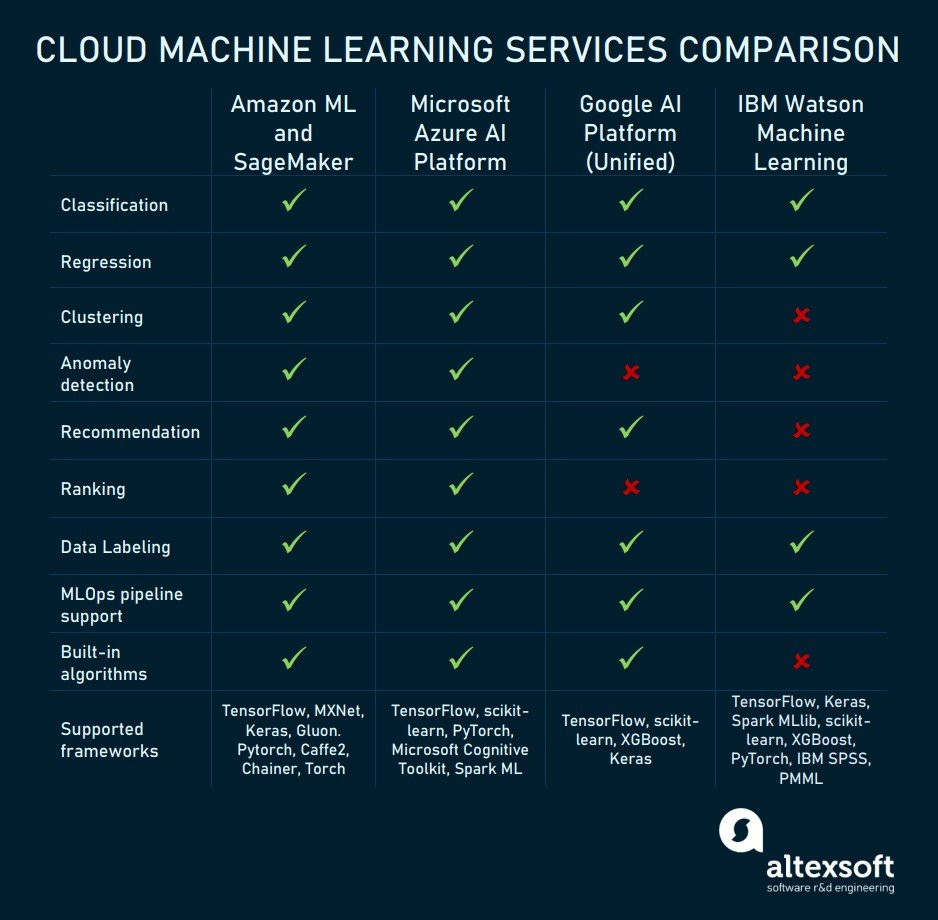
\includegraphics[width=150mm]{./appendices/mlaas-comparison}
    \caption{Machine learning as a Service comparison.~\cite{altexsoft2021mlaas}
    \label{fig:mlaas-comparison}}
\end{figure}

Amazon's new SageMaker service
has replaced the old Amazon Machine Learning service,
and is very much like Azure Machine Learning service
produced by Microsoft.
Compared to SageMaker and Azure, the
Google AI Platform is missing anomaly detection and ranking abilities.
IBM Watson has even less features,
as demonstrated in table~\ref{fig:mlaas-comparison}.~\cite{altexsoft2021mlaas}

Azure, however,
has one major advantage compared to SageMaker and other competitors,
which is the UI environment of ML Studio.
Most of the MLaaS providers' solutions
have some sort of no-code to low-code design features
which makes pipeline designing easy.
Azure ML Studio lets the developer design and deploy
full ML pipelines with drag-and-drop user interface.~\cite{altexsoft2021mlaas,microsoft2022azureml}

\begin{figure}[htb]
    \centering
    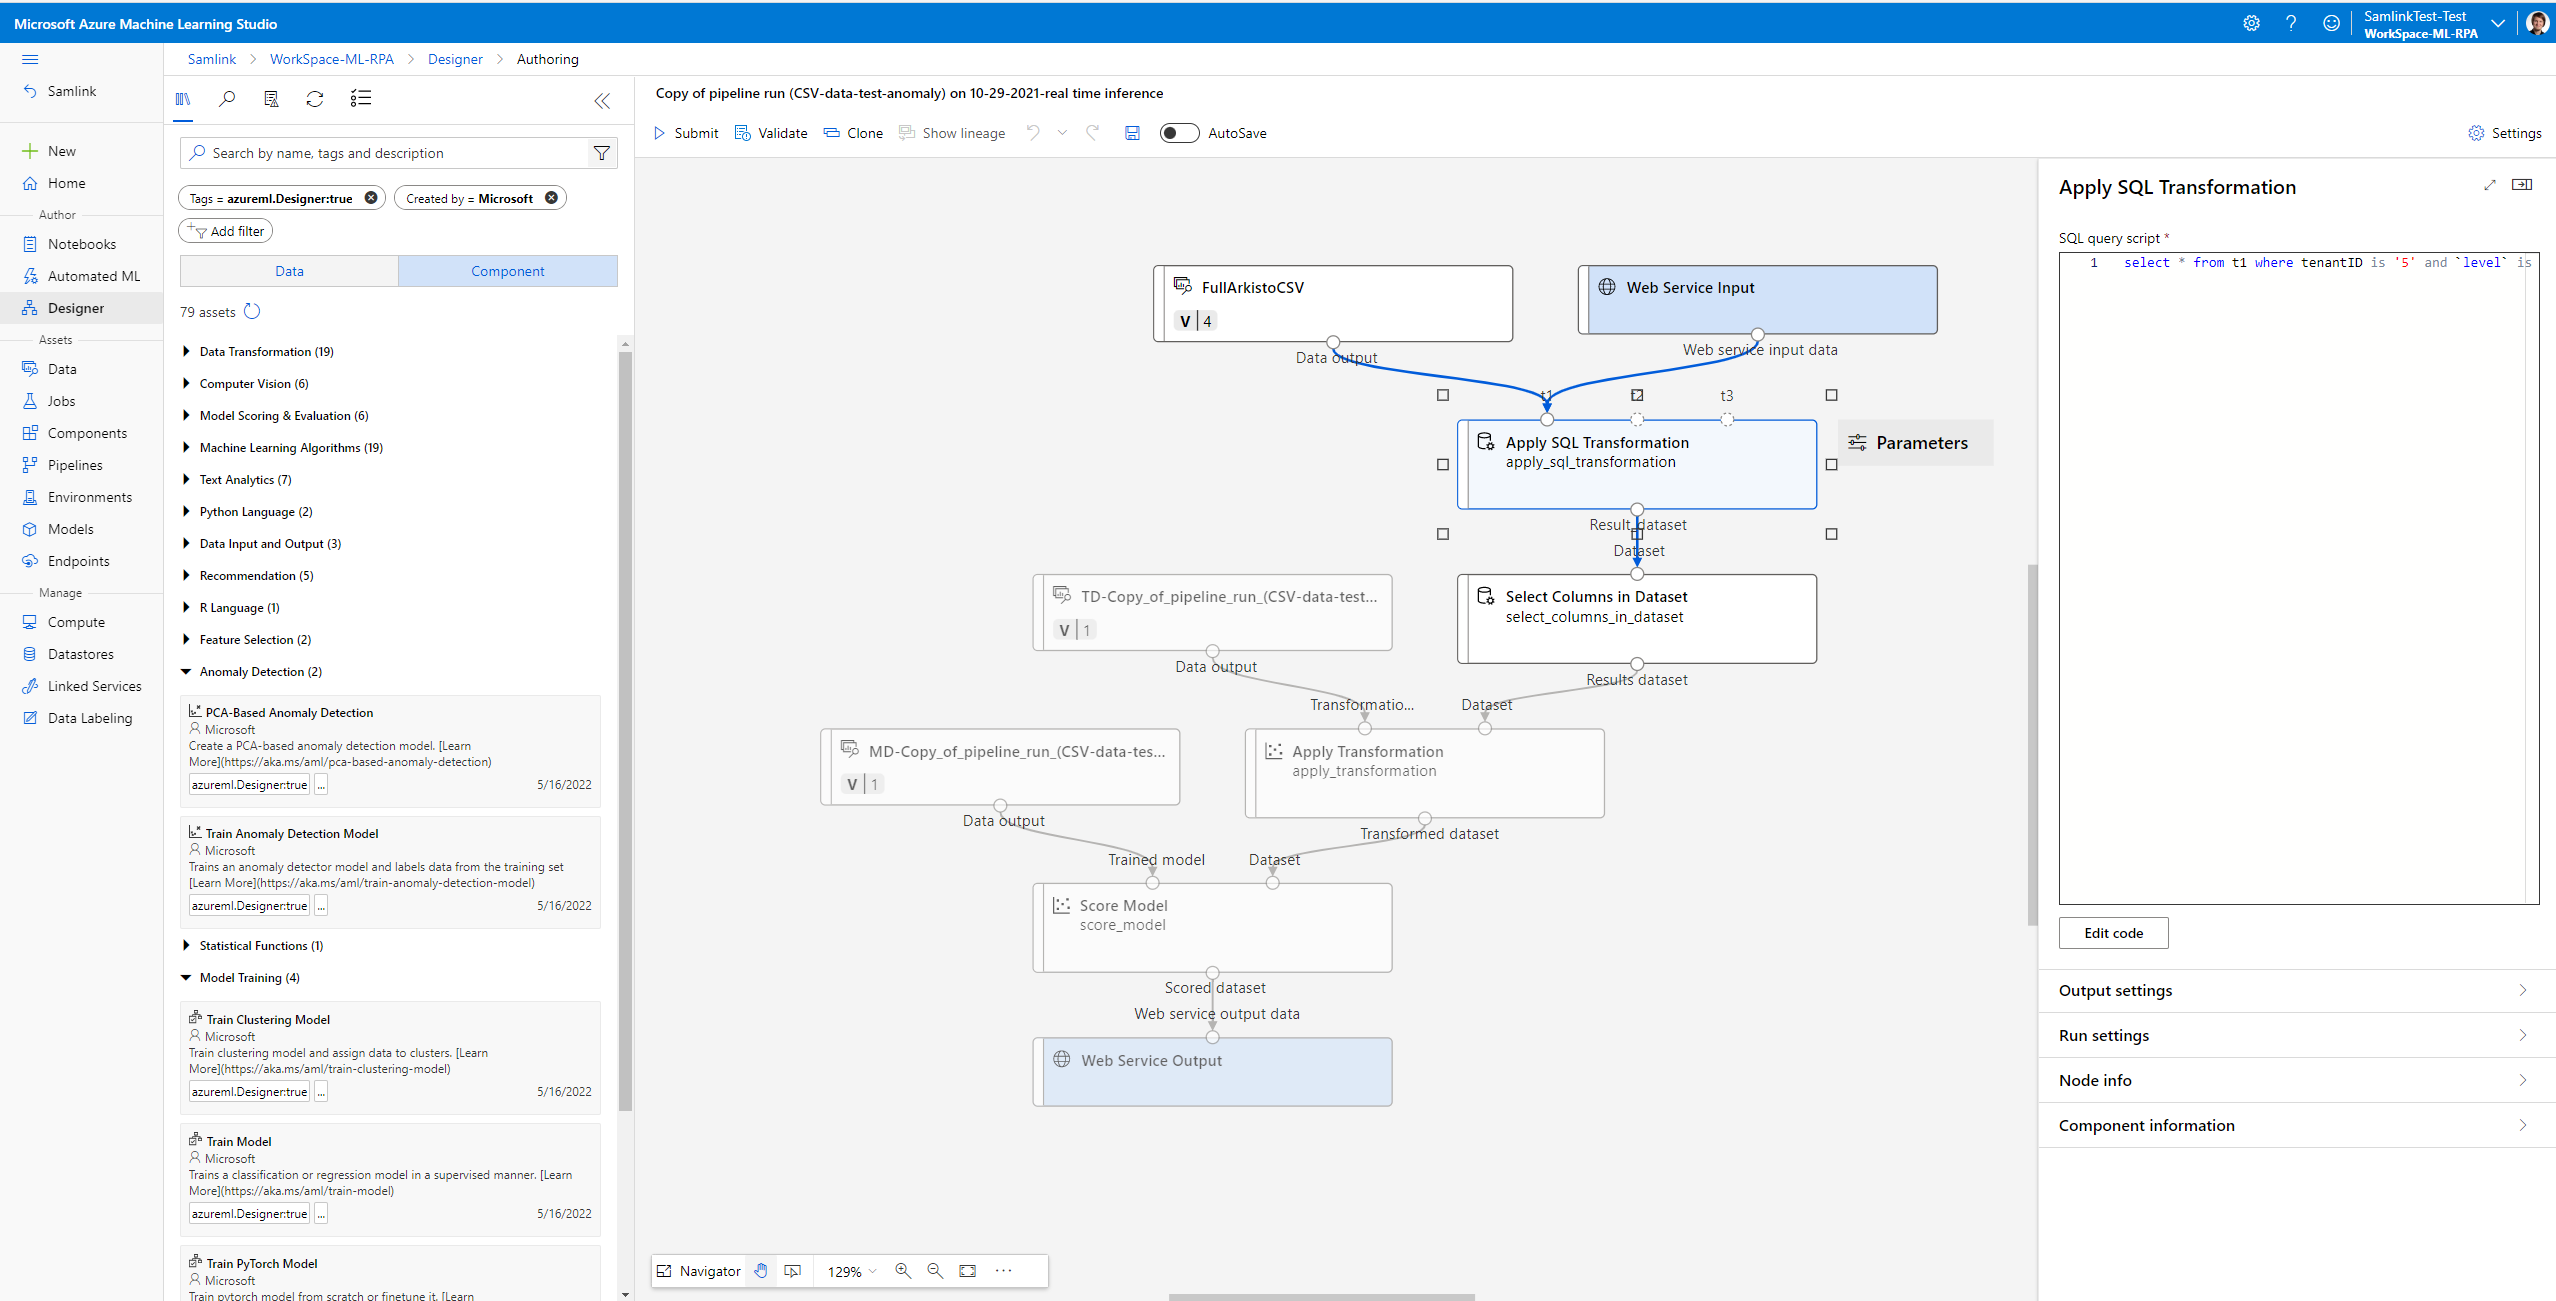
\includegraphics[width=150mm]{./appendices/azure-ml-studio-example}
    \caption{With drag-and-drop pipeline designer
    it is easy to get started with ML programming in Azure ML Studio,
    and visualizing the process helps understand all pipeline components
    and their relations to each other.
    \label{fig:azure-ml-studio-example}}
\end{figure}

Each component in the pipeline designer can be tuned
to certain extent.
ML Studio has a predefined set of ready algorithms to use.
An example of Azure ML Studio interface
is shown in figure~\ref{fig:azure-ml-studio-example}.
Data to the ML Studio environment
can be imported from local storage,
but also from various other Azure services
such as storage accounts with table and blob data.
Trained ML pipeline can be published as a cloud endpoint
and inserted into a wider operation chain
combining it with other Azure services,
like data storages and cloud computing resources.
This allows the designer to use ML computing capabilities
with existing production environments
utilizing services such as IoT, API, or Kubernetes.


%% ************************************************************************************************************

\subsection{Regression analysis}\label{subsec:bg-regression-ml}

Regression analysis is a typical approach in statistical science,
and thus, in machine learning too.
Algorithms based on regression analysis
are used to find relationships between a set of variables,
providing the means to \enquote{predict values of one variable
when given values of the others}
making them a fundamental component in the ML field.~\cite{merriam2022regression}

Regression algorithms intend to create a mathematical model
that explains the relations of the data.
This usually means an algebraic equation
which can be generalized in the following form,
\begin{equation}
    \label{eqn:general-regression-model}
    Y = f(X_{m},\beta_{p})+\epsilon
\end{equation}
where Y is the data feature we are looking to find relation to,
$f$ is some function of $m$ independent variables $(X_{m})$,
and $p$ coefficients $(\beta_{p})$.
$X_{m}$ can be opened as $X_{1},...,X_{m}$,
and $\beta_{p}$ as $\beta_{1},...,\beta_{p}$.
Note, that $m$ and $p$ do not have to be equal.
A single $X_{i}$ refers to a value of $i$th data row.
The $\epsilon$ refers to error term.
The goal is to determine the coefficients $\beta_{p}$
in order to find a model that explains the data.~\cite{freund2006regression}

As an example,
one of the best known principles for coefficient value solving
is the least square principle,
which aims to minimize the sum of squared errors (SSE).
The smaller the $SSE$ is,
the closer each data point is to the suggested model,
and the better the model explains the data
and can be used to make predictions.
The equation to solve in the least square principle
derived from the generalized form,
\begin{equation}
    \label{eqn:sum-of-squared-errors}
    SSE = \Sigma\epsilon^{2} = \Sigma[(Y-f(X_{1},...,X_{m},\beta_{1},...,\beta_{p}))]^{2}.
\end{equation}
Exact solution for this does not usually exist
as there can be more coefficients than independent variables $(p>m)$,
and minimizing the $SSE$ does not always result into a linear equation.
This is typically the case in ML,
and thus the model must be found
by iterative search process.
As mentioned in the section~\ref{subsec:bg-machine-learning},
this is what algorithms are build for.

To improve the efficiency of algorithm calculations,
the general regression model can be converted into matrix form.
The same function in equation~\ref{eqn:general-regression-model}
can thus be represented as,
\begin{equation}
    Y = XB+E
\end{equation}
where $Y$ is an $n\times1$ matrix of values in the data,
$X$ is an $n\times(m+1)$ matrix of independent variables,
$B$ is an $(m+1)\times1$ matrix of unknown coefficient parameters,
and finally, $E$ is an $n\times1$ matrix of error parameters.
Thus, the equation of squared errors (equation~\ref{eqn:sum-of-squared-errors})
that is to be minimized can be written as
\begin{equation}
    E^{T}E = (Y-XB)^{T}(Y-XB) = Y^{T}Y-2B^{T}X^{T}Y+B^{T}X^{T}XB.
\end{equation}
In order to minimize this, we can take the derivative of matrix $B$,
\begin{equation}
    \frac{\partial(E^{T}E)}{\partial B} = -2X^{T}Y + 2X^{T}XB.
\end{equation}
Equating to zero gives the solutions of coefficient parameters
\begin{equation}
    \hat{B} = (X^{T}X)^{-1}X^{T}Y.
\end{equation}

Ultimately,
there usually is no one perfect model to describe real world data.
As an example,
the function $f$ in the general regression model
can describe the relation of $X_{i}$ and $\beta_{i}$ as a product of both terms.
This would mean, that
\begin{equation}
    f(X_{1},...,X_{m},\beta_{1},...,\beta_{m})=\beta_{0}+\beta_{1}x_{1}+...+\beta_{m}x_{m}
\end{equation}
which would be a linear regression model.
Example of an algorithm using this method
is visualized in figure ~\ref{fig:linear-regression-example}.
However,
real world problems cannot always be explained with a linear model.
Fitting a polynomial curve to the data
may improve the results of regression to a certain degree,
but it also has its limits.

\begin{figure}[htb]
    \centering
    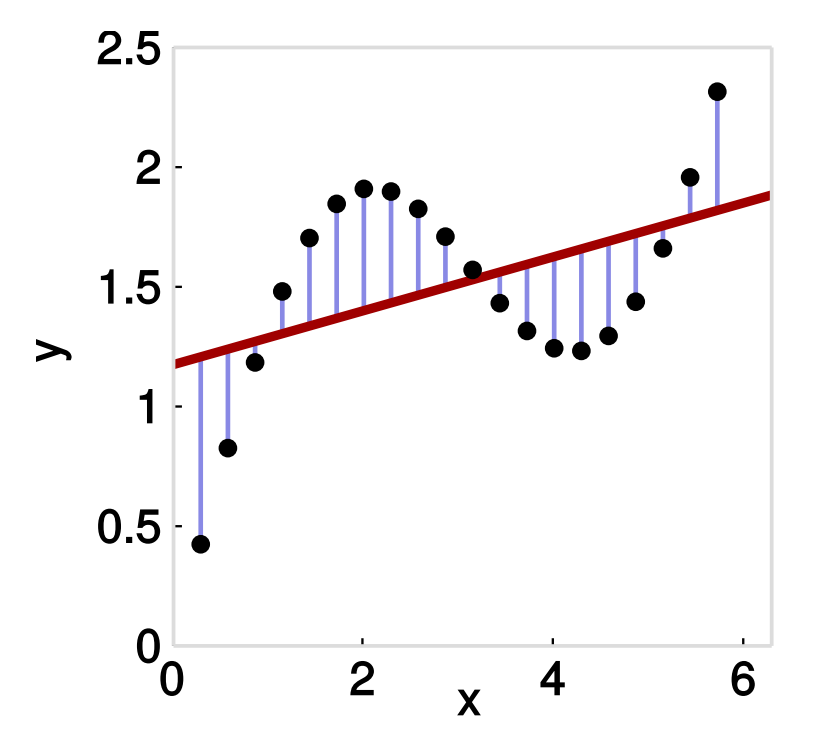
\includegraphics[width=0.5\textwidth]{./appendices/linear-regression}
    \caption{Linear least squares algorithm.
    Algorithm tries to fit a linear model (red line) on the data points,
        represented by the black dots,
        by minimizing the difference between all the data points
        and the model estimate.~\cite{stulp2015many}
        \label{fig:linear-regression-example}}
\end{figure}

Consider an algorithm that tries to keep a car
driving on a straight road in its lane.
The model output is how much we should turn the steering wheel
based on how much we are off from the straight line.
We might have constant parameters such as
wind effect, continuous error of the wheel axes, and tilt of the road.
However,
we also have parameters that change over time
and are dependent on other factors,
such as the weight of the car,
and the temperature and wear of the tires.
Therefore, with the same location at the road,
same car and same weather conditions,
our result could be different
depending on how long has been driven before the current moment
which affects the tire temperature and thus pressure.
Finding a model that best fits the data
depends also on the type of problem.
There are numerous algorithms to suit different situations,
and usually the best algorithm can be found
only by trial and error.


%% ************************************************************************************************************

\subsection{PCA-based anomaly detection}\label{subsec:bg-pca-ada}

Principal Component Analysis, or PCA,
is a machine learning technique
used to analyze data and explain the variance in it.
PCA analyzes data with multiple variables
and looks for correlations among them.
The final output PCA gives
is a new feature space,
\ie a smaller set of features (variables),
called \textit{principal components}.~\cite{azure2022pca}

In other words,
PCA works by reducing the dimensionality of the data.
First,
data must be standardized
so that the mean of each variable is zero
and the scale of each feature is the same.
\begin{equation}
    Standardized\; data\; point = \frac{data\; point\; value - mean\; value\; of\; the\; feature}{standard\; deviation\; of\; the\; feature}
\end{equation}
In practice,
the data points of each variable, or column,
is shifted so that their center is at 0
and the scale is adjusted to match all the variables.

Next, a covariance matrix for all the columns is determined.
As it is known,
covariance value between variables (or dimensions)
is calculated with
\begin{equation}
    cov(X,Y) = \frac{\Sigma_{i=1}^{n}(X_{i}-\bar{X})(Y_{i}-\bar{Y})}{(n-1)}
\end{equation}
where $X$ and $Y$ are different columns or variables,
$\bar{X}$ and $\bar{Y}$ their mean values (which both are zero after standardization),
$n$ is the number of rows or values in the data,
and so $X_{i}$ is the $i$th data point in the column $X$.~\cite{smith2002tutorial}

Covariance matrix is formed
by calculating the covariance value between each of the dimensions (including self).
For example,
for 3 dimensional data with dimensions $x$, $y$, and $z$, the
covariance matrix would be
\begin{equation}
    C =
    \begin{pmatrix}
        cov(x,x) & cov(x,y) & cov(x,z) \\
        cov(y,x) & cov(y,y) & cov(y,z) \\
        cov(z,x) & cov(z,y) & cov(z,z)
    \end{pmatrix}.
\end{equation}
Generally,
the covariance matrix for $n$ dimensions would then be, of course
\begin{equation}
    C =
    \begin{pmatrix}
        cov(1,1)    & \cdots    & cov(1,n)    \\
        \vdots      & \ddots    & \vdots        \\
        cov(n,1)    & \cdots    & cov(n,n)
    \end{pmatrix}.
\end{equation}

Next, we find the eigenvectors and eigenvalues
for the square-shaped covariance matrix.
As defined,
for $n\times n$ dimensional matrix $A$,
if exists a vector $x$ that satisfies
\begin{equation}
    Ax = \lambda x,
\end{equation}
where $\lambda$ is a scalar value,
such vector $x$ is an \textit{eigenvector} of matrix $A$,
and $\lambda$ is an \textit{eigenvalue},
forming the \textit{eigenpair} of $(\lambda,x)$.~\cite{borm2012numerical}

Eigenvectors have a property,
that either a matrix has zero of them,
or there are $n$ eigenvectors for $n\times n$ dimensional matrix.
Because in this case the eigenvectors are for the covariance matrix of the original (standardized) data,
they actually create a new feature space made of principal components.
More over,
eigenvalues describe their importance,
so that the greater the eigenvalue is,
the more significant the eigenvector is describing the original data
in principal component feature space.
When finding eigenpairs,
we actually find the largest possible variance in the data.
Each eigenvector describes a principal component
that is a linear combination of the original variables.
In figure ~\ref{fig:pca-example} we can see an example of
how eigenvectors of the covariance matrix define a new axis system
or new feature dimensions.~\cite{zhu2019dimension}
Each eigenvector, or a principal component,
is perpendicular with one another.
Thus, the data can be represented
in the new axis system formed by eigenvectors.

\begin{figure}[htb]
    \centering
    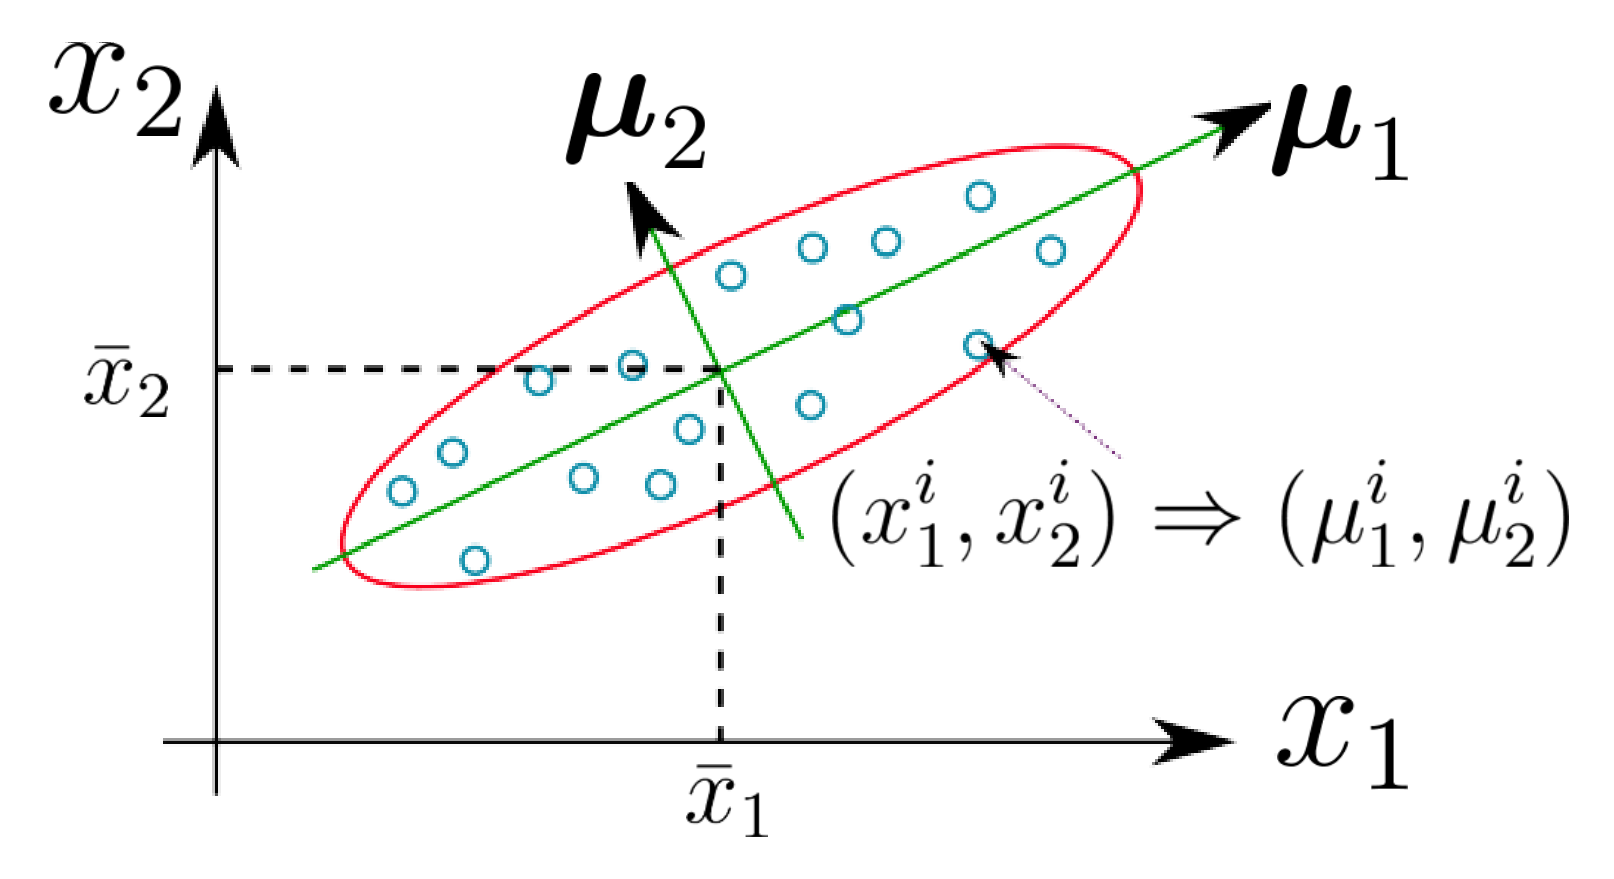
\includegraphics[width=0.7\textwidth]{./appendices/pca-example}
    \caption{Principal components form a new axis system.
    In this two dimensional example,
        eigenvectors $\mu_{1}$ and $\mu_{2}$ of the covariance matrix
        define new feature dimensions.
        Thus, data point $(x_{1}^{i},x_{2}^{i})$ of dimensions $x_{1}$ and $x_{2}$
        can be presented as a point $(\mu_{1}^{i},\mu_{2}^{i})$ of the dimensions $\mu_{1}$ and $\mu_{2}$.
        The origin point of each principal component axis is at the mean values of the data ($\bar{x}_{1}$ and $\bar{x}_{2}$)
        as the data is standardized.
        ~\cite{zhu2019dimension}
        \label{fig:pca-example}}
\end{figure}

By comparing the eigenvalues,
we can determine a set of eigenvectors,
or principal components,
that form a new feature space with fewer dimensions than the original data,
without losing a significant amount of information.
We can calculate a comparison value for each eigenvalue $\lambda_{i}$ with
\begin{equation}
    Percentage\; of\; variance = \frac{\lambda_{i}}{\Sigma\lambda}\cdot100
\end{equation}
Organized from highest to lowest,
we can make a scree plot to visualize the eigenvalue ratios
for all principal component.
Example of an 8 dimensional data
(which thus has 8 principal components),
with their eigenvalue variances ordered
can be seen in figure~\ref{fig:pc-variance-values}.

\begin{figure}[htb]
    \centering
    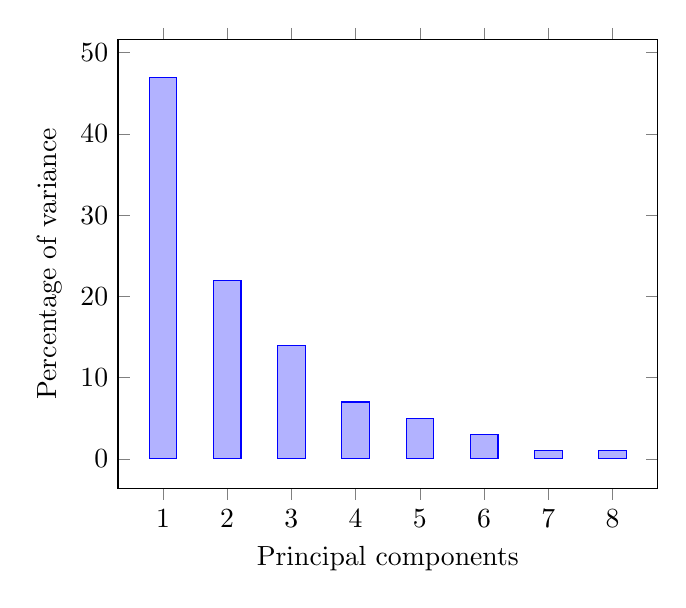
\begin{tikzpicture}
        \begin{axis} [
            ybar,
            ylabel={Percentage of variance},
            xlabel={Principal components},
            symbolic x coords={1,2,3,4,5,6,7,8},
            xtick=data
        ]
            \addplot coordinates {
                (1,47)
                (2,22)
                (3,14)
                (4,7)
                (5,5)
                (6,3)
                (7,1)
                (8,1)
            };
        \end{axis}
    \end{tikzpicture}
\caption{Significance of principal components.
In this example, eigenvalues, or the variance of each principal component,
    are ordered on a scree plot.
    Values are first converted to a percentage of the sum of all values
    in order to visualize both their relationship to each other
    and their total share of information held by the corresponding eigenvectors.
    \label{fig:pc-variance-values}}
\end{figure}

Practically,
as principal component space describes the data
and eigenvalues describe the importance of each component,
the percentage of variance is the portion of the total information each principal component holds.
Simply put,
in our example in figure~\ref{fig:pc-variance-values},
the first two principal components hold almost 70\% of the original information,
the first three over 80\%,
and the last seven hold less than 20\% of the information.
Thus,
by creating a new data set using the first three components,
we can keep 80\% of the information
while reducing the dimensions from 8 to 3,
which would be significant improvement
in terms of needed computing resources.
The amount of top principal components we choose to keep
depends on the situation,
but one guideline is to select all components
that describe more than a single variable's worth of information.
For our 8 dimensional example,
that would mean $1/8$th, or $12.5\%$,
meaning that we would select top 3 principal components
and discard the rest that are under $12.5\%$ of variance.
The remaining vectors form a new matrix
called \textit{feature vector}:
\begin{equation}
    Feature\; vector\; (F) = (x_{1} x_{2} ... x_{p})
\end{equation}
where $x_{i}$ is the $i$th eigenvector or feature component we chose to keep,
and $p$ is the amount of them, where $p<n$, $n$ being the original amount of dimensions of the data.

Finally,
we reorient our data from the original axes
to the space defined by the principal components
with the following equation:
\begin{equation}
    Final\; data = F^{T} A^{T}
\end{equation}
where $A$ is the original data set with standardized data,
which is transposed as well as the feature vector multiplying it.\cite{jaadi2021pca,holland2008principal,smith2002tutorial}

With principal components describing the distribution and variance of the data majority,
we can use PCA to detect anomalies.
This is done by analyzing each input
and computing its
\enquote{projection on the eigenvectors,
    together with a normalized reconstruction error.
    The normalized error is used as the anomaly score.
    The higher the error, the more anomalous the instance is}~\cite{azure2022pca}.
Normalized error means,
that each anomaly score is between zero and one.
Figure~\ref{fig:pca-nutshell} illustrates the steps
from data standardizing to PCA reconstruction error calculating.

\begin{figure}[htb]
    \centering
    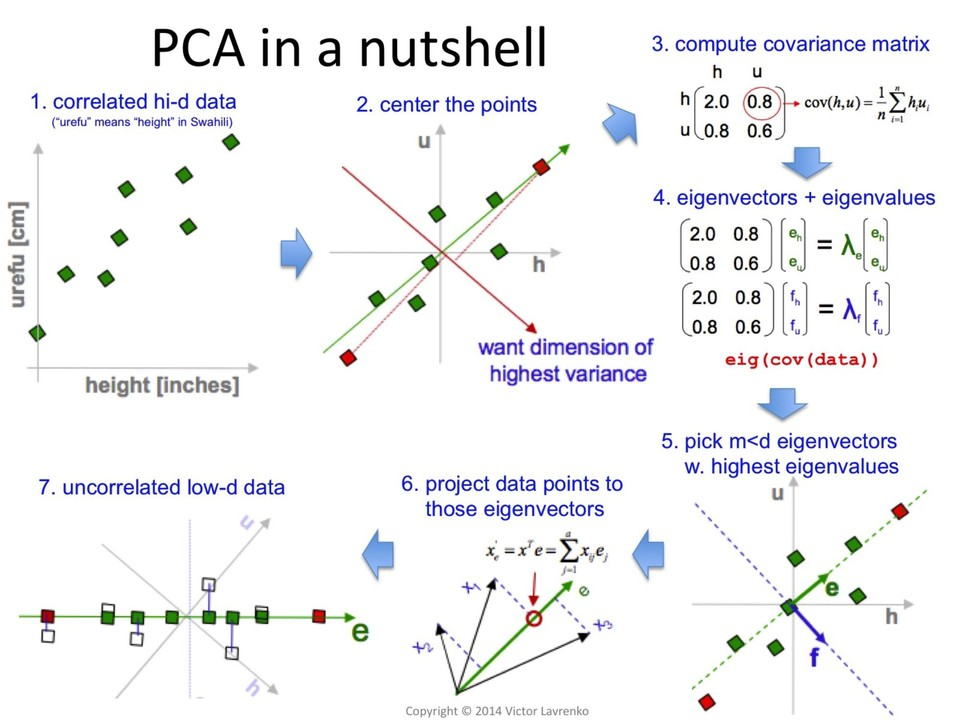
\includegraphics[width=\textwidth]{./appendices/pca-nutshell}
    \caption{PCA anomaly detection explained step by step.
    The normalized reconstruction error is the final anomaly probability score.
        \label{fig:pca-nutshell}}
\end{figure}


%% ............................................................................................................

\subsection{Other anomaly detection algorithms}\label{bg-other-ada}

Azure ML Studio has
also another anomaly detection algorithm to use besides the PCA-based one.
This module is called One-Class Support Vector Machine.
However,
it was not usable in the renewed ML Studio environment,
but was only available in the \textit{classic} Azure ML Studio.
In addition,
this module was not deemed suitable in our case,
as the documentation mentioned that
\enquote{The dataset that you use for training
can contain all or mostly normal cases.}
Because the content of the data used did not meet this requirement,
the usage possibilities of this component were not investigated.~\cite{azure2021oneclasssvm}
To limit the scope of this study to reasonable proportions,
we will not discuss other anomaly detection algorithms (ADAs) further.

%% ************************************************************************************************************

\subsection{N-gram features and feature hashing}\label{subsec:bg-ngram-features-and-hashing}

As discussed before,
features are the key elements in ML algorithm training.
As textual input does not have any meaning to computers by itself,
it is necessary to create a connection between words and features for algorithm.
In ML training,
one typical approach is to convert textual input into numerical features.
For example, by creating a dictionary of words used in the input
and assigning each word an identification number,
we can express sentences as a count of certain words used.
In addition,
words include meanings not only individually but also
with relation to each other and with their order.
For example,
words "success without errors"
has the opposite meaning than "errors without success"
where same words exist in a different order.
We can add more information for the algorithm
by creating word pairs and groups in the dictionary.
These groups are referred to as word grams,
where \textbf{n} in n-gram refers to the maximum number of words
in a group of consecutive words in the input sentence.~\cite{furnkranz1998study}

Example of n-gram composition of a sentence can be seen
in the table~\ref{tab:bg-n-gram-example}.
Usually,
the unnecessary stop words are removed from the text
(such as "the"),
as they don't bring any additional meaning to words or sentence.
One word grams are called \textit{unigrams},
two word grams \textit{bigrams}, \etc.
To compose the sentence \textit{"Lorem ipsum dolor sit amet, quisquam est, qui dolor ipsum qui dolor sit amet"}
with different n-gram dictionaries,
we could make, for example,
the following representation with unigram dictionary:
\begin{equation}
    1,2,3,4,5,6,7,8,3,2,8,3,4,5
\end{equation}
where each number represents the index of a word in a unigram dictionary from table~\ref{tab:bg-n-gram-example}.

\begin{table}[htb]
    \begin{tabularx}{\textwidth}{|L{0.1\textwidth}|L{0.17\textwidth}|L{0.25\textwidth}|Y|}
        \hline
        \textbf{Index} &
        \textbf{Unigrams} &
        \textbf{Bigrams} &
        \textbf{Trigrams}
        \\ \hline
        1	&	lorem       &	lorem ipsum     &	lorem ipsum dolor  \\ \hline
        2	&	ipsum       &	ipsum dolor     &	ipsum dolor sit  \\ \hline
        3	&	dolor       &	dolor sit       &	dolor sit amet  \\ \hline
        4	&	sit         &	sit amet        &	sit amet quisquam  \\ \hline
        5	&	amet        &	amet quisquam   &	amet quisquam est  \\ \hline
        6	&	quisquam    &   quisquam est    &	quisquam est qui \\ \hline
        7	&	est         &   est qui 		&	est qui dolor  \\ \hline
        8	&	qui         &   qui dolor 	    &	qui dolor ipsum \\ \hline
        9	&	            &  	dolor ipsum 	&   dolor ipsum qui \\ \hline
        10	&	            &  	ipsum qui 		&   ipsum qui dolor \\ \hline
        11	&	            &  	 				&   qui dolor sit \\ \hline
    \end{tabularx}
    \caption{N-gram feature extraction from a sentence
    "Lorem ipsum dolor sit amet, quisquam est, qui dolor ipsum qui dolor sit amet".}
    \label{tab:bg-n-gram-example}
\end{table}

N-gram representation of the text
streamlines the algorithm processing of textual features.
However,
each new word creates a new feature
when converting text to n-grams.
This happens,
because in order to present text as numerical features,
we need to create a new feature space out of the n-gram dictionary.
Consider our unigram dictionary from the previous example.
This would convert one text column into 8 unigram features,
as seen in table~\ref{tab:bg-n-gram-features}.

\begin{table}[htb]\small
\begin{tabularx}{\textwidth}{|L{0.07\textwidth}|L{0.09\textwidth}|L{0.09\textwidth}|L{0.08\textwidth}|L{0.07\textwidth}|L{0.07\textwidth}|Y|L{0.07\textwidth}|L{0.07\textwidth}|}
    \hline
    \textbf{row} &
    \textbf{lorem} &
    \textbf{ipsum} &
    \textbf{dolor} &
    \textbf{sit}	&
    \textbf{amet} &
    \textbf{quisquam} &
    \textbf{est} &
    \textbf{qui}
    \\ \hline
    1	&	1	&	2	&	3	&	1	&	2	&	1	&	1	&	2 \\ \hline
\end{tabularx}
\caption{One row with a textual feature presented as n-gram feature transformation.
Each new word in the n-gram dictionary adds a new feature and thus a dimension to the data.}
\label{tab:bg-n-gram-features}
\end{table}

As the number of word grams in a dictionary can increase significantly
in complex input cases,
it is necessary to limit the resource usage by decreasing the features that are analyzed.
One way to compress the dimensions is to use
feature hashing for n-gram features.~\cite{azure2021fhash}
This means that instead of pure n-gram features representing a single n-gram instance,
we use hashed value of several n-grams
thus reducing the amount of features.
Hashing can be done in different ways,
for example by multiplying each original feature together,
or calculating a weight value based on the frequency of each feature.
As a drawback,
the amount of information might also get reduced as the data is "compressed".
The more dimensions are compressed into hashing values,
the more information is bound to be lost,
but this way we can include more features for algorithm training
without significant resource demands.~\cite{caragea2012protein,shi2009hash}

%% ************************************************************************************************************

\subsection{Robotic process automation}\label{subsec:bg-rpa}

Robotic process automation, or RPA,
is used to automate mechanical tasks executed on computer software.
Usually it operates on the UI level
and can be used to repeat meaningful functions
instead of mechanical actions.
For example, with screen recording macros,
only mouse position at the screen and actual pressing of the keyboard
is recorded and repeated.
RPA automation, however,
is able to repeat the functionalities those actions trigger,
such as inputting text to a certain named field on the UI,
or logging in with a given username and password
regardless of the location of those fields on the layout.~\cite{tripathi2018learning}

In Samlink,
an RPA technology called UiPath is used as a base of RPA operations.
A central coordinating system called "UiPath Orchestrator"
supervises the RPA processes.
RPA process is executed by following
an "RPA automation",
a predefined operation instruction build by RPA developer.
The software responsible for the automation execution
is called "RPA agent".
Agents are located in the "workstations",
where a single agent is running in one workstation.
Each agent executes one automation at a time,
given by the Orchestrator,
and communicates with Orchestrator during the execution.
This hierarchy is visualized in figure~\ref{fig:rpa-hierarchy}.

\begin{figure}[htb]
    \centering
    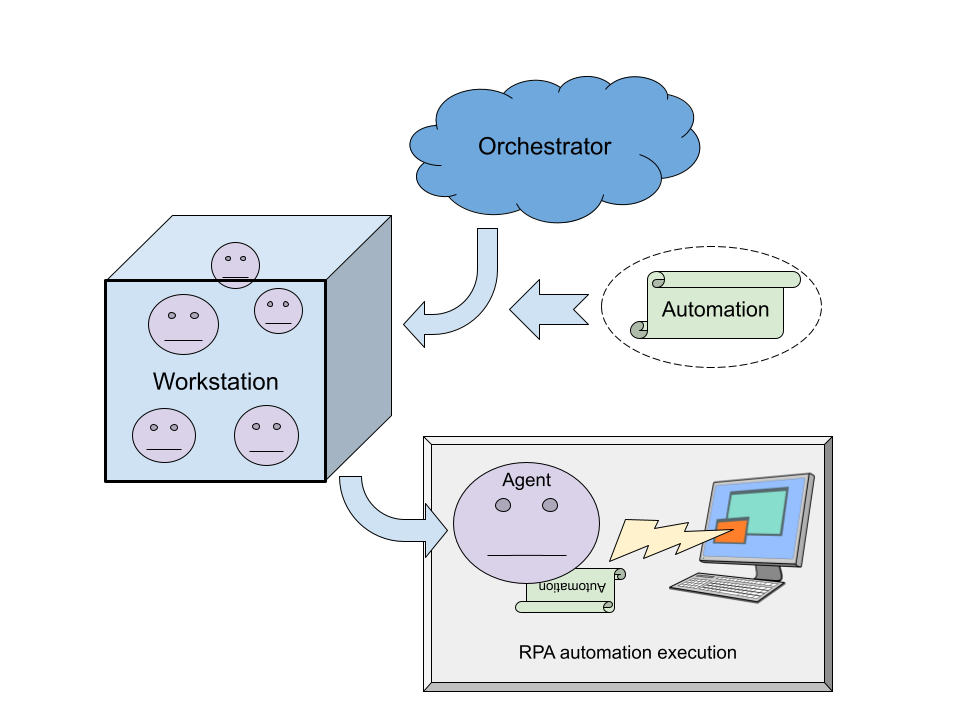
\includegraphics[width=\textwidth,]{./appendices/RPA-hierarchy}
    \caption{Hierarchy of RPA components explaining the terms and their relations.
    \label{fig:rpa-hierarchy}}
\end{figure}


%% ************************************************************************************************************

\subsection{Data sensitivity}\label{subsec:bg-data-sensitivity}

During this study,
it was necessary to make sure no sensitive data
was moved out of the production environment.
This was mostly due to restrictions imposed by GDPR\@.
In order to maintain the data security,
the data had to be anonymized
before it could be exported to the cloud environment.
After anonymization,
the data would not include any information
that can be connected to real individuals.
Three different anonymization methods were considered,
which were pseudonymization, k-anonymization and full anonymization.

Pseudonymization refers to a method
where sensitive information is de-identified.
This means,
that each sensitive piece of information
is replaced with an encrypted value
so that no information is lost
but a human cannot identify individuals
when reading the data.
Encryption and de-identification
could be reversed, \ie data could be re-identified,
with a decryption key which tells a computer
how to convert the replaced value back to the original form.
As machine learning algorithms do not care about the meanings
behind personal identification information,
such as phone numbers or addresses,
pseudonymization would preserve the information in the data unchanged
for ML algorithms to use so that no information would be lost.~\cite{noumeir2007pseudonymization}

As pseudonymization is a reversible operation with an encryption key,
it is not the safest way to anonymize the data
because the encryption key leaking is always a risk.
K-anonymization is the next step in securing the data sensitivity.
Excluding all unique identifiers such as full name or social security number,
information like home street, age, workplace or last name
are not on their own enough to identify a certain individual,
but combined they can single out a person.
K-anonymization is an unreversable anonymization approach
where identifying information is generalized
to mask individuals into a crowd.
With k-anonymization,
an algorithm replaces single informative details
with more general variants,
for instance,
address to hometown or age to age range.
K-anonymization loses information
as it cannot be reversed.
If personal information is essential for the use case of the ML algorithm,
this method weakens the algorithm results.~\cite{byun2007efficient}

Eventually,
due to high customer data sensitivity and strict data safety policies,
it was determined that individual information in the log data used in this study
was not relevant for connecting the log events to technical support ticket timestamps.
Thus full anonymization was decided to execute on the log data.
This way,
each personal information was replaced with a general token
disclosing only what type of information (phone number, email address \etc) was anonymized.
Frankly,
it is not certain if identifiable personal data would have improved the algorithm results,
but because corresponding support ticket data
was stripped from all other information except timestamps,
any possible connections between personal data in logs and in tickets
were lost nonetheless.

Data anonymization was executed in the production environment
with PowerShell script.
Several predefined identification features were searched with
regular expression (or regex) patterns and replaced with
default keys.
Anonymization scripts and the data format
is described in more detail in the section~\ref{subsec:meth-data-anonymization}.


%% ************************************************************************************************************

\subsection{Log data analysis and anomaly detection with ML}\label{subsec:bg-log-data-analysis-and-anomaly-detection-with-ml}

Using machine learning for log data analysis
is not a new field of study.~\cite{rantala2019applying,allagi2019analysis,kondo2017early,cao2017machine}
The key issue tends to be the format of the log data
which shifts the dilemma to natural language processing.
Some studies also combine anomaly detection using machine learning
to log data analysis.~\cite{liu2019loganomaly, zhang2019robust}
Comparing existing studies to our case
raises at least one major suggestion for improvement:
log data refining.

When log data has a consistent format,
multiple different algorithms can be utilized
for anomaly detection and log analysis.
Log events can be clustered
and different types of events can be counted
if the amount of types is finite and known.~\cite{liu2019loganomaly}

If training data already have information
we wish to teach the algorithm to forecast (\ie data is labeled),
combining the results of the log data analysis to external features
is more feasible.
With labeled data,
supervised learning methods can improve the results of the algorithm forecast abilities.
~\cite{rantala2019applying}

As explained in the section~\ref{subsec:meth-efecte-ticket-data},
data features connected to anomaly detection results
are pure datetime values.
With more insight into ticket data properties than just timestamps,
ML algorithms could be able to extract more valuable information
from the log data.


\clearpage